\documentclass[tikz, margin=5mm]{standalone}

%%% This file contains definitions of shapes and nodes used
%%% for a recipe workflow
%%% Author       : Oliver Czoske
%%% Created      : 2021-03-03
%%% Last Changed : 2021-03-03
%%% Changes:
%%%

\usetikzlibrary{
  shapes.misc,
  positioning,
  calc,
  arrows.meta}

%% All connecting lines have an arrow
\tikzset{
  connection_arrow/.style={->, >=Latex[open], thick}
}

%% Start and stop buttons (black disks, stop with ring)
%% These are pics, use as
%%         \pic (name) [above of=..] {picname};
\tikzset{
  start/.pic = {
    \node (-m) at (0, 0){};
    \filldraw [fill=black] (0, 0) circle (0.2);
  }
}

\tikzset{
  stop/.pic = {
    \node (-m) at (0, 0){};
    \node (-t) at (0, -0.3){};
    \filldraw [fill=black] (0, 0) circle(0.2);
    \draw[black] (0, 0) circle (0.3);
  }
}


%%%% Various boxes and their colours
%%%% These are nodes, use as
%%%% \node (name) [type, location]  {text};

\definecolor{stepcolor}{RGB}{210,169,188}
\definecolor{rawcolor}{RGB}{205,205,205}
\definecolor{externalcolor}{RGB}{183,255,255}
\definecolor{calibcolor}{RGB}{255,250,216}
\definecolor{calproductcolor}{RGB}{185,184,237}
\definecolor{qcproductcolor}{RGB}{255,201,165}
\definecolor{sciproductcolor}{RGB}{197,219,183}
\definecolor{framecolor}{RGB}{127,13,65}

\tikzset{
  %% template : the template(s) that trigger(s) the recipe
  template/.style={
    rectangle,
    draw=black,
    minimum width=4.0cm,
    minimum height=0.5cm,
    align=center
  },
  %% input : the input files
  input/.style={
    rectangle,
    fill=rawcolor,
    minimum width=4.0cm,
    minimum height=0.75cm,
%     text width=3cm,
    align=center
  },
  %% calib : calibration input
  calib/.style={
    rectangle,
    fill=calibcolor,
    minimum width=4.0cm,
    minimum height=0.75cm,
%     text width=3cm,
    align=center
  },
  %% external : external input
  external/.style={
    rectangle,
    fill=externalcolor,
    minimum width=4.0cm,
    minimum height=0.75cm,
%     text width=3.5cm,
    align=center
  },
  %% params : parameters
  params/.style={
    rectangle,
    draw=red,
    thick,
    minimum width=4.0cm,
    minimum height=0.75cm,
%     text width=3cm,
    align=center
  },
  %% redstep : a reduction step
  %%      ("step" is predefined and can't be used)
  redstep/.style={
    rectangle,
    rounded corners=0.2cm,
    fill=stepcolor,   %%% define colour!
    minimum width=4.0cm,
    minimum height=1cm,
%     text width=3cm,
    align=center
  },
  %% connection : connection to input or output
  connection/.style={
    circle,
    fill=black,
    minimum size=0.15cm,
    inner sep=0pt
  },
  %% sciproduct : a science product
  sciproduct/.style={
    rectangle,
    fill=sciproductcolor,
    minimum width=4.0cm,
    minimum height=0.75cm,
%     text width=3.5cm,
    align=center
  },
  %% calproduct : a calibration product
  calproduct/.style={
    rectangle,
    fill=calproductcolor,
    minimum width=4.0cm,
    minimum height=0.75cm,
%     text width=3.5cm,
    align=center
  },
  %% frame : frame around the recipe
  %% This is a path, use as
  %%    \draw [frame] (upper left) rectangle (lower right);
  frame/.style={framecolor, very thick, dashed}
}


\begin{document}

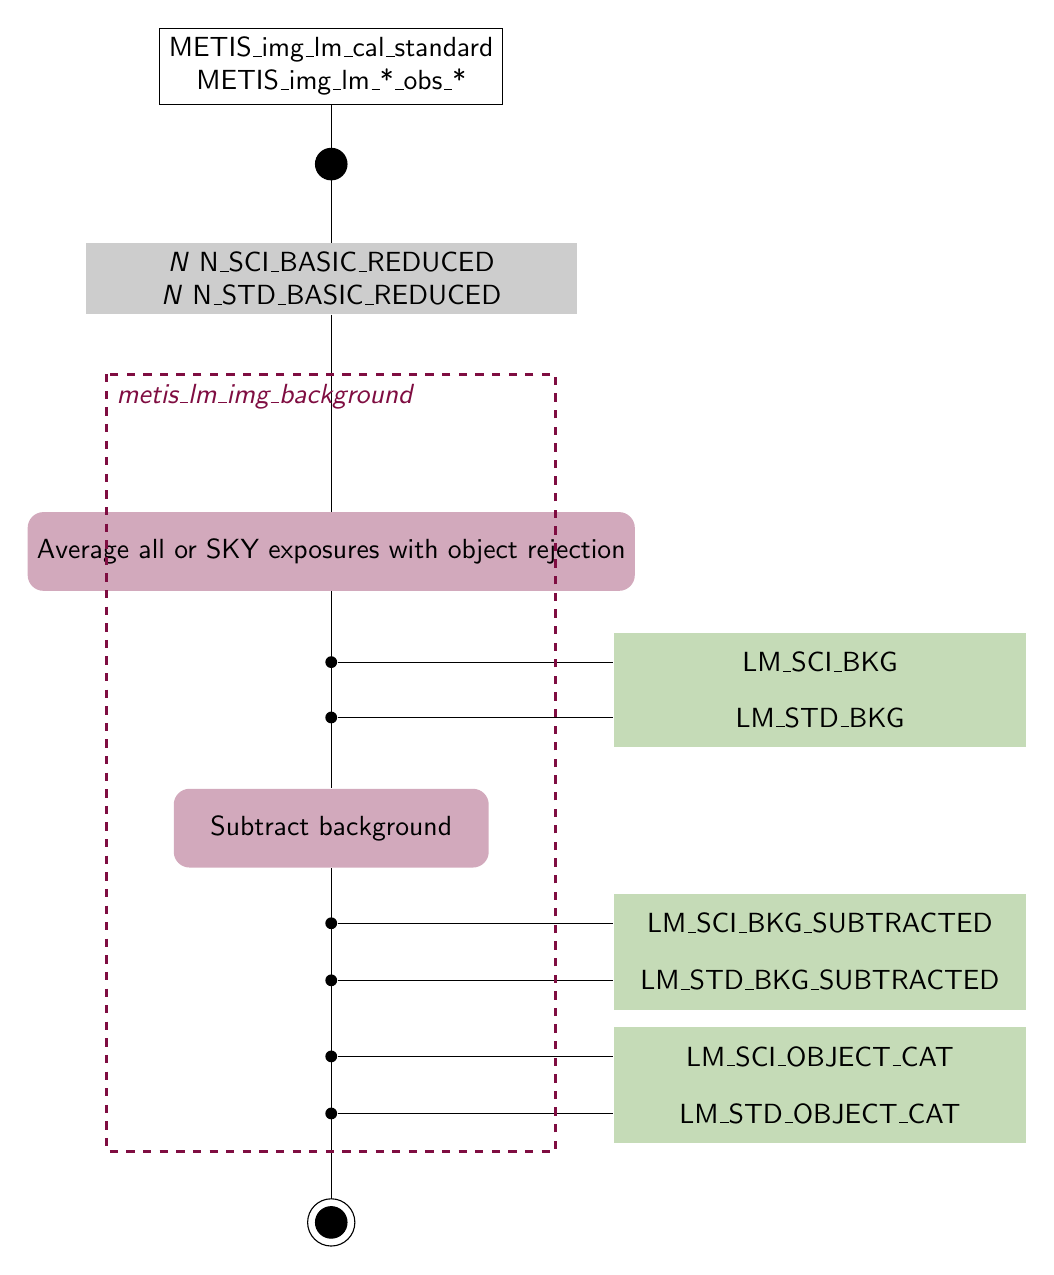
\begin{tikzpicture}
  [x=1cm,
  y=-1cm,
  align=center,
  node distance=2cm and 3.5cm]
  \sffamily

  %% template names
  \node (template) [template] {%
    METIS\_img\_lm\_cal\_standard\\
    METIS\_img\_lm\_*\_obs\_*};

  \pic (start)[below=0.75cm of template]{start};


  %% input box
  \node (input) [below=0.75cm of start-m, input, text width=6cm] {%
    \textsl{N} N\_SCI\_BASIC\_REDUCED\\
    \textsl{N} N\_STD\_BASIC\_REDUCED};


  %% algorithm steps
  \node (step1) [below=2.5cm of input, redstep]{%
    Average all or SKY exposures with object rejection};

  \node (step2) [below=2.5cm of step1, redstep]{%
    Subtract background};

  \pic (stop) [below=4.5cm of step2] {stop};


  %% Connections
  \draw (template) -- (input);
  \draw (input) -- (step1);
  \draw (step1) -- (step2);
  \draw (step2) -- (stop-t);


  %% External data

  % External input

  % External output
  \node (dot_sci_bg) [connection] at
    ($(step1)!0.4!(step2)$){};
  \node (sci_bg) [right=of dot_sci_bg, sciproduct, text width=5cm]{%
    LM\_SCI\_BKG};
  \draw (dot_sci_bg) -- (sci_bg);

  \node (dot_std_bg) [connection] at
    ($(step1)!0.6!(step2)$){};
  \node (std_bg) [right=of dot_std_bg, sciproduct, text width=5cm]{%
    LM\_STD\_BKG};
  \draw (dot_std_bg) -- (std_bg);


  \node (dot_sci_bg_sub) [connection] at
    ($(step2)!0.25!(stop-t)$){};
  \node (sci_bg_sub) [right=of dot_sci_bg_sub, sciproduct, text width=5cm]{%
    LM\_SCI\_BKG\_SUBTRACTED};
  \draw (dot_sci_bg_sub) -- (sci_bg_sub);

  \node (dot_std_bg_sub) [connection] at
    ($(step2)!0.4!(stop-t)$){};
  \node (std_bg_sub) [right=of dot_std_bg_sub, sciproduct, text width=5cm]{%
    LM\_STD\_BKG\_SUBTRACTED};
  \draw (dot_std_bg_sub) -- (std_bg_sub);


  \node (dot_sci_obj_cat) [connection] at
    ($(step2)!0.6!(stop-t)$){};
  \node (sci_obj_cat) [right=of dot_sci_obj_cat, sciproduct, text width=5cm]{%
    LM\_SCI\_OBJECT\_CAT};
  \draw (dot_sci_obj_cat) -- (sci_obj_cat);

  \node (dot_std_obj_cat) [connection] at
    ($(step2)!0.75!(stop-t)$){};
  \node (std_obj_cat) [right=of dot_std_obj_cat, sciproduct, text width=5cm]{%
    LM\_STD\_OBJECT\_CAT};
  \draw (dot_std_obj_cat) -- (std_obj_cat);


  %% Frame around recipe
  \draw [frame] ($(input)!0.35!(step1) -(2.85,0)$) rectangle
  ($(step2)!0.85!(stop-t) + (2.85,0)$);
  \node [framecolor, anchor=north west] at
  ($(input)!0.35!(step1) - (2.85,0)$){%
    \textsl{metis\_lm\_img\_background}};


\end{tikzpicture}

\end{document}
